\chapter{Related Work}

\section{Ad-hoc methods}
	Simple distortion methods are applied to the image privacy protection field such as pixelation and blurring. The pixelation method subsamples the image and the blurring method smoothes images with some filters like Gaussian filter or average filter ~\cite{Agrawal09,Boyle00}. Both by destorying the original image information, pixelation and blurring make a trade between privacy information and image quality. Although these two methods are widely used in practical situations like TV interviews, they suffer from the same risk proposed in ~\cite{Newton05} called parrot attack. General face recognition algorithms figure out the identity by computing the similarity between the target image and database images. Blur and pixelation destory the target image information so that the target image is not similar to any image in database. Parrot attack would preprocess all the database images with pixelation or blurring, then applies face recognition algorithms to pixelated or blurred images so that target images and database images are preprocessed with the similar procedures. 

	\par
	Two more de-identificaiton methods are introduced in ~\cite{Winkler14}: blanking and encryption. The intuitive blanking method in face de-identificaiton is to cut the face region off and replace the region with black color. It also could be extended to paint the region of interest, like face, with background images  ~\cite{inpaint09,Qureshi09}. Compared with other de-identification methods introduced before, encryption has the advantage in recovery ~\cite{Boult05}. With a proper key, the encrypted image is always available to be decrypted so that the image remains useful even if it is covered by a snowboard. These two methods cover image information including both identity and facial expressions. It is the balance between privacy and data utilization that should be the key point in face de-identification. Protecting the identity privacy while preserving facial expressions simultanously is the purpose of our research. 
	
	\par
	Dufaux ~\cite{dufaux08} introduced a privacy protection method using in video sequence by scrambling the locations of pixels in a rectangle range. By controling the range size, different degrees of fuzzy results could be produced. It is possible to recover the original image information if the scrambling order is recorded. Essentially, the scrambling method is a kind of encryption with the permutation order as the encryption key. Scrambling method overcomes other traditional encryption methods in original information preserving. If the scrambling range is in proper size, the original information is still understandable. In another word, scrambling also trades privacy protection with data utility. The images shown in Figure \ref{adhoc_example} retriving from ~\cite{dufaux08} illustrate the examples of different de-identification methods above. 
	% whether place four images here
	\begin{figure}[!htb]
		  \centering
		  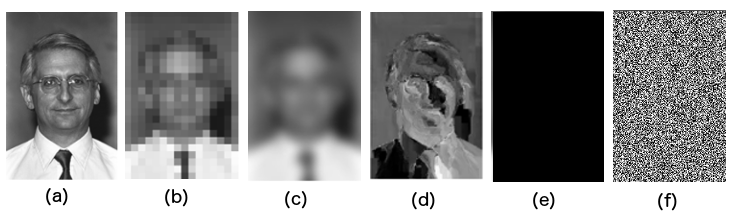
\includegraphics[width=0.9\textwidth]{figure/adhoc.png} 
		  \caption{(a) the origianl image; (b) pixelation; (c) blurring; (d) scrambling; (e) blanking; (f) encryption}
		  \label{adhoc_example}
	\end{figure}

	\par
	There are still some interesting and simple methods in face de-identification field such as cartooning and face swapping. Converting a real image into cartooning one is a developed technology. Erdélyi ~\cite{erdely14} applied this technology in de-identification area by applying edge detector and mean-shift algorithm in the real image so that the pixels with similar colors would be assign the same value. It is intuitive that cartooning method is able to thwart automatic face recognition algorithms. However, it is hardly deceive a human. Face swapping is also a popular and simple method to de-identify face images. The simplest explanation of this idea is to replace one person's face with another one's. The research in ~\cite{CAVE08} shows the face swapping result could be photorealistic. As a improved version of face swapping method, S. Mosaddegh etc. ~\cite{Mosa14} composes a new face to replace the original one by taking several donors' face parts, thus making the synthetic face contain several persons' characters. 

	\par
	As a summation, the previous de-identification methods are all trade-offs between privacy protection and data utility preservation. When processed by the previous introduced methods, the original face image information would be damaged to protect identity but also erase some data utility such as expressions, gender. In another word, the previous introduced methods protect identity privacy information by destorying all the original image information, which definitely destory the data utility simultaneously. 

\section{K-anonymity based methods}
	K-anonymity is a model proposed by ~\cite{Sweeney02} to solve the problem that a data holder releases a version of private data with scientific guarantees that the individuals involved can not be re-identified while the data remain pratically useful. Suppose one indivual's data is a tuple, this method requires that the released data contain at least k same tuples so that the re-identification ratio for each individual is lower than $\frac{1}{k}$. Originally not specifically designed for face images, the k-anonymity model is applied in various kinds of data. The following table shows the k-anonymity model used in an example of citizen's information from United States. \newline
		\begin{table}[!htb]
		\centering
			\begin{tabular}{|c|c|c|c|c|}
				\hline
				\textbf{Race} & \textbf{Birth} & \textbf{Gender} & \textbf{ZIP} & \textbf{Problem} \\
				\hline
				Black & 1965 & m & 0214* & short breath \\
				\hline
				Black & 1965 & m & 0214* & chest pain \\
				\hline
				Black & 1965 & f & 0213* & hypertension \\
				\hline
				Black & 1965 & f & 0213* & hypertension \\
				\hline
				Black & 1964 & f & 0213* & obesity \\
				\hline
				Black & 1964 & f & 0213* & chest pain \\
				\hline
				White & 1964 & m & 0213* & chest pain \\
				\hline
				White & 1964 & m & 0213* & obesity \\
				\hline
				White & 1964 & m & 0213* & short breath \\
				\hline
				White & 1967 & m & 0213* & chest pain \\
				\hline
				White & 1967 & m & 0213* & chest pain \\
				\hline
			\end{tabular}
			\caption{A K-anonymity example in text information, $k = 2$ ~\cite{Sweeney02}} 
		\end{table}	

		The number k from above example is 2 which means the possibility ratio of re-identify any individual from the database is less than $\frac{1}{2}$ judging from \{Race, Birth, Gender, ZIP\}. In another word, at least 2 same tuples in \{Race, Birth, Gender, ZIP, Problem\} would appear in this database. If this is the version of released database, it is possible to get statistic information from this but impossible to match each tuple with specific citizens. Therefore, it is claimed this could keep a ballance from privacy protection and data utility preservation.  
	
	\subsection{\emph{k-Same} algorithm}

	E. Newton firstly applied the K-anonymity method to privacy protectin by de-identifying face images in 2005 ~\cite{Newton05}. The experiment was set in a person specific face image database, which means only one face image for each individual is included. Claiming that ad-hoc methods, like pixelation, blurring, are not able to protect privacy, E. Newton introduced two new approaches based on K-anonymity model: \emph{k-Same-Pixel} and \emph{k-Same-Eigen}. These two algorithms are tested in the person specific database that contains only one image for each person. 

	For any one face image from $A$ the person specific database, the process of \emph{k-Same-Pixel} is:
	\begin{itemize}
		\item Select $k$ face images that are closest to $A$ including A itself
		\item Take the average of these $k$ images $A_{new}$ by averaging the sum of pixels
		\item Replace the original image $A$ with $A_{new}$
		\item Repeat the first step if the recognition ratio of A is higher than $\frac{1}{k}$
	\end{itemize}
	The only difference between \emph{k-Same-Pixel} and \emph{k-Same-Eigen} is the later one would take an average image from eigen faces. In mathematics, the eigen face images, composed of eigen values and eigen vectors of original images, are also called projected images, which are computed by PCA (Principle Component Analysis). 

	Images provided by \emph{k-Same-Eigen} have a blurred effect compared to those from \emph{k-Same-Pixel} because the projected images used in \emph{k-Same-Eigen} retain only the most important characteristics. Less important components have been removed during the computation of eigen values and eigen vectors.

	Compared to ad-hoc methods, \emph{k-Same-Pixel} and \emph{k-Same-Eigen} are able to combat the parrot attack. It is an improvement in the privacy protection. However, as illustrated before, the key point in face de-identificaiton is to keep the ballance between privacy protection and data utility preservation. The data utility of face images from \emph{k-Same-Pixel} and \emph{k-Same-Eigen} would be discussed. 
 	
 	\subsection{\emph{k-Same-M}}
 	This \emph{k-Same-M} algorithm is designed to overcome an obvious shortcoming of \emph{k-Same-Pixel} and \emph{k-Same-Eigen}. Since the previous introduced k-Same algorithms average the de-identified images based on pixels directly and different faces are with various sizes, the alignment between faces are not always perfect correct. Therefore, the de-identified face image may contain ghost artifacts. As shown in Fig.~\ref{ghostFace} ~\cite{Gross08}, the appearance of de-identified face images are deeply fuzzy. Although the de-identified images are able to combat automatic face recognition algorithms, the results also lose many other informations like expressions. Even a normal human could not figure out the expressions in the results. Hence, we claim that the k-Same algorithm fail to keep the balance between data privacy and data utility. 
	 	\begin{figure}[!htb]
			  \centering
			  \includegraphics[width=0.8\textwidth]{figure/ghost.png} 
			  \caption{Ghost face images produced by k-Same algorithm}
			  \label{ghostFace}
		\end{figure}
 	The M in \emph{k-Same-M} represents Model. 

	\subsection{\emph{k-Same-Select}}
	
	General solutions model face shape and appearance separately. 

	\subsection{Shortcomings of k-Same framework}

	\section{Multi-factor Model}